\documentclass[addpoints,12pt]{exam}\usepackage[]{graphicx}\usepackage[]{color}
%% maxwidth is the original width if it is less than linewidth
%% otherwise use linewidth (to make sure the graphics do not exceed the margin)
\makeatletter
\def\maxwidth{ %
  \ifdim\Gin@nat@width>\linewidth
    \linewidth
  \else
    \Gin@nat@width
  \fi
}
\makeatother

\definecolor{fgcolor}{rgb}{0.345, 0.345, 0.345}
\newcommand{\hlnum}[1]{\textcolor[rgb]{0.686,0.059,0.569}{#1}}%
\newcommand{\hlstr}[1]{\textcolor[rgb]{0.192,0.494,0.8}{#1}}%
\newcommand{\hlcom}[1]{\textcolor[rgb]{0.678,0.584,0.686}{\textit{#1}}}%
\newcommand{\hlopt}[1]{\textcolor[rgb]{0,0,0}{#1}}%
\newcommand{\hlstd}[1]{\textcolor[rgb]{0.345,0.345,0.345}{#1}}%
\newcommand{\hlkwa}[1]{\textcolor[rgb]{0.161,0.373,0.58}{\textbf{#1}}}%
\newcommand{\hlkwb}[1]{\textcolor[rgb]{0.69,0.353,0.396}{#1}}%
\newcommand{\hlkwc}[1]{\textcolor[rgb]{0.333,0.667,0.333}{#1}}%
\newcommand{\hlkwd}[1]{\textcolor[rgb]{0.737,0.353,0.396}{\textbf{#1}}}%


\makeatletter
\newenvironment{kframe}{%
 \def\at@end@of@kframe{}%
 \ifinner\ifhmode%
  \def\at@end@of@kframe{\end{minipage}}%
  \begin{minipage}{\columnwidth}%
 \fi\fi%
 \def\FrameCommand##1{\hskip\@totalleftmargin \hskip-\fboxsep
 \colorbox{shadecolor}{##1}\hskip-\fboxsep
     % There is no \\@totalrightmargin, so:
     \hskip-\linewidth \hskip-\@totalleftmargin \hskip\columnwidth}%
 \MakeFramed {\advance\hsize-\width
   \@totalleftmargin\z@ \linewidth\hsize
   \@setminipage}}%
 {\par\unskip\endMakeFramed%
 \at@end@of@kframe}
\makeatother

\definecolor{shadecolor}{rgb}{.97, .97, .97}
\definecolor{messagecolor}{rgb}{0, 0, 0}
\definecolor{warningcolor}{rgb}{1, 0, 1}
\definecolor{errorcolor}{rgb}{1, 0, 0}
\newenvironment{knitrout}{}{} % an empty environment to be redefined in TeX

\usepackage{alltt}
\usepackage{amsmath, amssymb}
\linespread{1.1}
\usepackage{hyperref}
\usepackage{enumerate}
\usepackage{multirow}

%-------------------DON'T CHANGE---------------------%
%The following is needed to prevent a conflict between knitr and the exam class involving the package ``framed.''

%-------------------DON'T CHANGE---------------------%



%This keeps images from being too big, centers them, and makes sure we use pdf images



%Change the default width of the output to fit within the solution boxes


\printanswers

%To include the answers use:
%  pdflatex "\def\showanswers{1} \input{thisfile.tex}"
%\ifdefined\showanswers
%  \printanswers
%\else
%  \noprintanswers
%\fi

\title{Problem Set (Week 4)}
\author{Econ 103}
\date{}
\IfFileExists{upquote.sty}{\usepackage{upquote}}{}
\begin{document}
\maketitle




%\section*{Part II -- Additional Problems}

\section*{Lecture 12}

Note: In the following five questions  $X_1, X_2 \sim \mbox{ iid } N(\mu, \sigma^2)$, $Y = (X_1 - \mu)/\sigma$, $Z = (X_2 - \mu)/\sigma$.

\begin{questions}

\question 
	\begin{parts}
		\part What is the distribution of $X_1 + X_2$?
			\begin{solution}
				$X_1 + X_2 \sim N(2\mu, 2\sigma^2)$
			\end{solution}
		\part Use R to calculate $P(X_1 + X_2 > 5)$ if $\mu = 5$ and $\sigma^2 = 50$.
			\begin{solution}
			In this case, $X_1 + X_2 \sim N(10, 100)$, hence
			\begin{eqnarray*}
				P(X_1 + X_2 > 5) &=& 1 - P(X_1 + X_2 \leq 5) \\
				&=& 1 - P\left(\frac{X_1 + X_2 - 10}{10} \leq \frac{5-10}{10}\right)\\
				&=& 1 - \mbox{\texttt{pnorm(-0.5)}}\\
				&\approx& 0.6914625
			\end{eqnarray*}
			Alternatively, we could use  \texttt{1- pnorm(5, mean = 10, sd = 10)}, which gives the same result.
			\end{solution}
		\part Use R to calculate the 10th percentile of the distribution of $X_1 + X_2$.
			\begin{solution}
				\texttt{qnorm(p = 0.1, mean = 10, sd = 10)} gives -2.815516.
			\end{solution}
	\end{parts}
%\question 
%	\begin{parts}
%		\part What is the distribution of $Y^2$?
%			\begin{solution}
%				As the sum of squares of one standard normal RV, $Y^2 \sim \chi^2(1)$.
%			\end{solution}
%		\part Use R to calculate $P(Y^2 \geq 1)$.
%			\begin{solution}
%				\begin{eqnarray*}
%					P(Y^2 \geq 1) = 1 - P(Y^2 \leq 1) = 1 -  \mbox{\texttt{pchisq(1, df = 1)}} \approx 0.3173105
%				\end{eqnarray*}
%			\end{solution}
%	\end{parts}
	
%\question
%	\begin{parts}
%		\part What is the distribution of $Y^2 + Z^2$?
%			\begin{solution}
%			Since this is the sum of squares of two independent standard normal random variables, $Y^2 + Z^2 \sim \chi^2(2)$.
%			\end{solution}
%		\part Use R to calculate the 95th percentile of the distribution of $Y^2 + Z^2$.
%			\begin{solution}
%				\texttt{qchisq(p = 0.95, df = 2)} gives 5.991465
%			\end{solution}
%	\end{parts}
\question 
	\begin{parts}
	\part What is the distribution of $Z/\sqrt{Y^2}$?
		\begin{solution}
			Since it is the ratio of a standard normal to the square root of an independent $\chi^2$ random variable divided by its degrees of freedom (in this case one), $Z/\sqrt{Y^2}\sim t(1)$.
		\end{solution}
	\part What value of $c$ satisfies $P(-c\ \leq Z/\sqrt{Y^2} \leq c )=0.95$?
		\begin{solution}
			By the symmetry of the $t$-distribution, it suffices to find the $97.5$th percentile (this allocates 2.5\% probability to the upper and lower tails).  The command \texttt{qt(p = 0.975, df = 1)} gives 12.7062, so $c \approx 12.7$. Alternatively, we could have calculated the 2.5th percentile: \texttt{qt(p = 0.025, df = 1)} gives -12.7062.
		\end{solution}
	\part How does the interval in part (b) compare to the corresponding interval for $Z$?
		\begin{solution}
		Since $Z$ is a standard normal RV, $P(-2\leq Z \leq 2) \approx 0.95$. We see that the interval for a $t(1)$ RV is \emph{much wider} than the corresponding interval for a standard normal. In other words, extreme outcomes are much more likely under the $t(1)$ distribution.
		\end{solution}
	\end{parts}
	
\question 
	\begin{parts}
		\part What is the distribution of $Y^2/Z^2$?
			\begin{solution}
				This is the ratio of two independent $\chi^2$ random variables, each divided by its degrees of freedom (in this case, one). Hence $Y^2/Z^2\sim F(1,1)$.
			\end{solution}
		\part Use R to calculate the 95th percentile of the distribution of $Y^2/Z^2$.
			\begin{solution}
				\texttt{qf(p = 0.95, df1 = 1, df2 = 1)} gives 161.4476
			\end{solution}
	\end{parts}

\section*{Lecture 13}


\question  In this question, you will use R to study the sampling distribution of the sample mean where we take as our population the heights of all students in Econ 103.
	\begin{parts}
		\part Load the class survey data used in R Tutorial \# 2, extract the height column and assign it to a variable called \texttt{height}. Use \texttt{!is.na} to remove all missing values from \texttt{height}.
\begin{solution}
\begin{knitrout}
\definecolor{shadecolor}{rgb}{0.969, 0.969, 0.969}\color{fgcolor}\begin{kframe}
\begin{alltt}
\hlstd{data.url} \hlkwb{<-} \hlstr{"http://www.ditraglia.com/econ103/old_survey.csv"}
\hlstd{survey} \hlkwb{<-} \hlkwd{read.csv}\hlstd{(data.url)}
\hlstd{height} \hlkwb{<-} \hlstd{survey}\hlopt{$}\hlstd{height}
\hlstd{height} \hlkwb{<-} \hlstd{height[}\hlopt{!}\hlkwd{is.na}\hlstd{(height)]}
\end{alltt}
\end{kframe}
\end{knitrout}
\end{solution}
  \part Make a histogram of height and calculate the mean height for students in the class. For the purposes of this exercise, these correspond to the \emph{population}.
\begin{solution}
\begin{knitrout}
\definecolor{shadecolor}{rgb}{0.969, 0.969, 0.969}\color{fgcolor}\begin{kframe}
\begin{alltt}
\hlkwd{hist}\hlstd{(height,} \hlkwc{main} \hlstd{=} \hlstr{'Population - All Econ 103 Students'}\hlstd{,}
     \hlkwc{xlab} \hlstd{=} \hlstr{'Height in Inches'}\hlstd{)}
\end{alltt}
\end{kframe}

{\centering 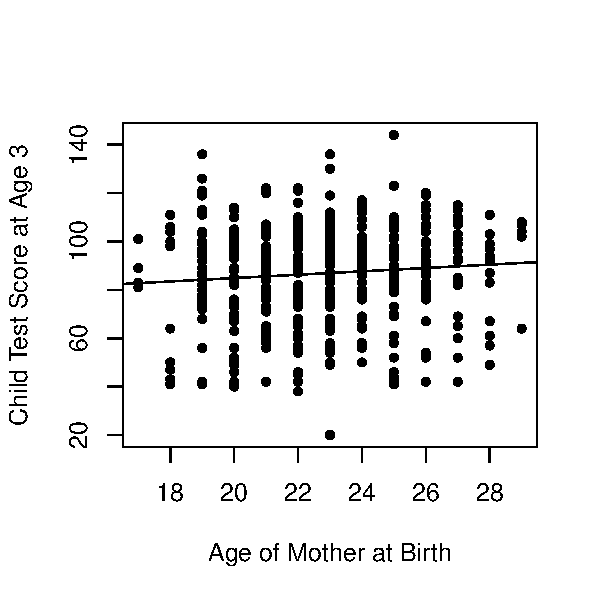
\includegraphics[width=\maxwidth]{figure/unnamed-chunk-5-1} 

}


\begin{kframe}\begin{alltt}
\hlkwd{mean}\hlstd{(height)}
\end{alltt}
\begin{verbatim}
## [1] 67.54545
\end{verbatim}
\end{kframe}
\end{knitrout}
\end{solution}
  \part Write a function that takes $n$ as its only input and returns the sample mean of an iid random sample of size n drawn from the vector \texttt{height}. Call this function \texttt{x.bar.draw}. [Hint: use \texttt{sample} with \texttt{replace = TRUE}.]
\begin{solution}
\begin{knitrout}
\definecolor{shadecolor}{rgb}{0.969, 0.969, 0.969}\color{fgcolor}\begin{kframe}
\begin{alltt}
\hlstd{x.bar.draw} \hlkwb{<-} \hlkwa{function}\hlstd{(}\hlkwc{n}\hlstd{)\{}

  \hlstd{sim} \hlkwb{<-} \hlkwd{sample}\hlstd{(height,} \hlkwc{size} \hlstd{= n,} \hlkwc{replace} \hlstd{=} \hlnum{TRUE}\hlstd{)}
  \hlkwd{return}\hlstd{(}\hlkwd{mean}\hlstd{(sim))}

\hlstd{\}}\hlcom{#END x.bar.draw}
\end{alltt}
\end{kframe}
\end{knitrout}
\end{solution}
  \part Test the function you wrote for part (d) by running it with \texttt{n = 10000}. What value do you get? Your answer should be approximately equal the population mean you calculated above. If it isn't, something is wrong with your code.
\begin{solution}
\begin{knitrout}
\definecolor{shadecolor}{rgb}{0.969, 0.969, 0.969}\color{fgcolor}\begin{kframe}
\begin{alltt}
\hlkwd{x.bar.draw}\hlstd{(}\hlnum{10000}\hlstd{)}
\end{alltt}
\begin{verbatim}
## [1] 67.4819
\end{verbatim}
\end{kframe}
\end{knitrout}
\end{solution}
%  \part Using the R function \texttt{replicate}, run your function \texttt{x.bar.draw} 10000 times with $n = 5$. Store the result in a vector called \texttt{x.bar.5}. Do the same for $n = 10, 20$ and $50$ and store the results as vectors \texttt{x.bar.10}, \texttt{x.bar.20} and \texttt{x.bar.50}
%\begin{solution}
%<<cache=TRUE>>=
%x.bar.5 <- replicate(10000, x.bar.draw(5))
%x.bar.10 <- replicate(10000, x.bar.draw(10))
%x.bar.20 <- replicate(10000, x.bar.draw(20))
%x.bar.50 <- replicate(10000, x.bar.draw(50))
%@
%\end{solution}
 % \part Calculate the mean and variance of \texttt{x.bar.5},\texttt{x.bar.10}, \texttt{x.bar.20} and \texttt{x.bar.50} and plot a histogram of each, being sure to label them.
%\begin{solution}
%<<>>=
%mean(x.bar.5)
%mean(x.bar.10)
%mean(x.bar.20)
%mean(x.bar.50)
%hist(x.bar.5)
%hist(x.bar.10)
%hist(x.bar.20)
%hist(x.bar.50)

%var(x.bar.5)
%var(x.bar.10)
%var(x.bar.20)
%var(x.bar.50)
%@
%\end{solution}
	\end{parts}


\section*{Lecture 14}

\question Textbook question: Chapter 7-18.
\begin{solution}
    \textbf{7-18}\\
    The point of this question is non-response bias: the people who respond are not representative of the population as a whole. Note that $P$ and $P^*$ as defined in this question \emph{do not correspond} to question 7-13. Our goal is to estimate the population proportion who will buy a computer. Using the table, we calculate the total number of people who will buy a computer as:
  $$0.02 \times 40 + 0.04\times 5 + 0.1\times 3 + 0.2\times 2 = 1.7 \mbox{ million}$$
which corresponds to a fraction $\pi^* = 1.7/50 = 0.034$. Again using the table, the number of people who will buy a computer \emph{among the sub-population who would respond} can be calculated as:
	$$0.02 \times 7 + 0.04\times 1 + 0.1\times 1 + 0.2\times 1 =  0.48 \mbox{ million}$$
which corresponds to a fraction $\pi = 0.48/10 = 0.048$. The point is that $\pi \neq \pi^*$. In other words, the proportion of people who would buy a computer \emph{differs} across people who would and would not respond to the phone survey. The estimator $P$ is based on calling 1000 people chosen at random and recording responses for \emph{only those who reply}. The proportion of people who will reply is $10/50 = 1/5$. Thus, $P$ will end up with a sample size of approximately $n=200$ individuals. These individuals correspond to the sub-population for which the proportion who would buy a computer is $\pi^* = 0.048$. In contrast, the estimator $P^*$ is based on calling $n^* = 100$ people chosen at random and then following up with these people repeatedly until \emph{all of them respond}. Thus, $P^*$ draws from the \emph{full population}, in which a proportion $\pi^* = 0.034$ of people will buy a computer. The \emph{true parameter} is $\pi^*$ since we want to estimate the \emph{overall} fraction of people who will buy a computer, \emph{not} the fraction of people who would buy a computer among those who are likely to respond to a telephone survey. Hence bias is calculated \emph{relative to} $\pi^*$. Variance is calculated \emph{relative to the mean of each sampling distribution}. For $P$ this mean is $\pi$ while for $P^*$ it is $\pi^*$. That is:
	\begin{eqnarray*}
		MSE(P) &=& \mbox{Bias}(P)^2 + Var(P) = (E[P] - \pi^*)^2 + E[(P - \pi)^2]\\
		&=& (\pi - \pi^*)^2 + E[(P - \pi)^2]\\
		&=&  (\pi - \pi^*)^2 + \pi(1-\pi)/n\\
		MSE(P^*)	&=& \mbox{Bias}(P^*)^2 + Var(P^*) = (\pi^* - \pi^*)^2 + E[(P^* - \pi^*)^2]\\
			&=& E[(P^* - \pi^*)^2] = \pi^*(1-\pi^*)/n^*
	\end{eqnarray*}
The estimator $P^*$ does not have any bias because of the follow-ups to ensure that everyone in the original random sample responds. However, since it is based on a smaller sample, we would expect it to have a higher variance. The question is how this trade-off comes out in the expressions for MSE. To find out, we simply plug in the values $\pi^* = 0.034$, $\pi = 0.048$, $n =200$ and $n^* = 100$. We find $MSE(P^*) \approx 0.000328$ and $MSE(P) \approx 0.000424$.
    \end{solution}
    
\section*{Lecture 15-16}

    \question For this question assume that we have a random sample from a normal distribution with unknown mean but \emph{known} variance.
    \begin{parts}
      \part Suppose that we have 36 observations, the sample mean is 5, and the population variance is 9. Construct a 95\% confidence interval for the population mean.
        \begin{solution}
        Since the population variance is 9, the population standard deviation is $3$. Hence, the desired confidence interval is
        $5 \pm 2 \times 3/\sqrt{36} = 5\pm 1 = (4,6)$
        \end{solution}
      \part Repeat the preceding with a population variance of 25 rather than 9. 
      \begin{solution}
      The population standard deviation becomes $5$ so the confidence interval becomes 
      $5 \pm 2 \times 5/\sqrt{36} = 5\pm 10/6 \approx  (3.3,6.7)$
      \end{solution}
      \part Repeat the preceding with a sample size of  25 rather than 36.
        \begin{solution}
              $5 \pm 2 \times 5/\sqrt{25} = 5\pm 2 = (3,7)$
        \end{solution}
    %  \part Repeat the preceding but construct a 50\% rather than 95\% confidence interval.
 %     \begin{solution}
  %    Here we need to use R to get the appropriate quantile:
%\begin{knitrout}
%\definecolor{shadecolor}{rgb}{0.969, 0.969, 0.969}\color{fgcolor}\begin{kframe}
%\begin{alltt}
%\hlstd{SE} \hlkwb{<-} \hlnum{5}\hlopt{/}\hlkwd{sqrt}\hlstd{(}\hlnum{25}\hlstd{)}
%\hlstd{ME} \hlkwb{<-} \hlkwd{qnorm}\hlstd{(}\hlnum{1} \hlopt{-} \hlnum{0.5}\hlopt{/}\hlnum{2}\hlstd{)} \hlopt{*} \hlstd{SE}
%\hlstd{Lower} \hlkwb{<-} \hlnum{5} \hlopt{-} \hlstd{ME}
%\hlstd{Upper} \hlkwb{<-} \hlnum{5} \hlopt{+} \hlstd{ME}
%\hlkwd{c}\hlstd{(Lower, Upper)}
%\end{alltt}
%\begin{verbatim}
%## [1] 4.326 5.674
%\end{verbatim}
%\end{kframe}
%\end{knitrout}
 %     \end{solution}
      \part Repeat the preceding but construct a 99\% rather than a 95\% confidence interval.
            \begin{solution}
      Again we use R to get the appropriate quantile:
\begin{knitrout}
\definecolor{shadecolor}{rgb}{0.969, 0.969, 0.969}\color{fgcolor}\begin{kframe}
\begin{alltt}
\hlstd{SE} \hlkwb{<-} \hlnum{5}\hlopt{/}\hlkwd{sqrt}\hlstd{(}\hlnum{25}\hlstd{)}
\hlstd{ME} \hlkwb{<-} \hlkwd{qnorm}\hlstd{(}\hlnum{1} \hlopt{-} \hlnum{0.01}\hlopt{/}\hlnum{2}\hlstd{)} \hlopt{*} \hlstd{SE}
\hlstd{Lower} \hlkwb{<-} \hlnum{5} \hlopt{-} \hlstd{ME}
\hlstd{Upper} \hlkwb{<-} \hlnum{5} \hlopt{+} \hlstd{ME}
\hlkwd{c}\hlstd{(Lower, Upper)}
\end{alltt}
\begin{verbatim}
## [1] 2.424 7.576
\end{verbatim}
\end{kframe}
\end{knitrout}
      \end{solution}
      \part How would you construct the confidence interval if the variance is \textit{unknown}? Explain what estimator you will use to approximate the variance and what distribution you will use to construct the interval. 
      \begin{solution}
      Since we do not know the population variance (standard deviation), we will use the sample variance (standard deviation) to construct the relevant random variable as in the lecture note. Then we will use t distribution with degrees of freedom $n=1 = 36-1$ to get the associated quantiles.
      \end{solution}
    \end{parts}

\end{questions}




\end{document}
